\documentclass[11pt,a4wide]{article}
\usepackage{verbatim}
\usepackage{listings}
\usepackage{graphicx}
\usepackage{a4wide}
\usepackage{color}
\usepackage[options]{SIunits}
\usepackage{amsmath}
\usepackage{amssymb}
\usepackage[dvips]{epsfig}
\usepackage[utf8]{inputenc}
\usepackage[OT1]{fontenc}
\usepackage{cite} % [2,3,4] --> [2--4]
\usepackage{shadow}
\usepackage{hyperref}

\setcounter{tocdepth}{2}
%
\lstset{language=c++}
\lstset{alsolanguage=[90]Fortran}
\lstset{basicstyle=\small}
\lstset{backgroundcolor=\color{white}}
\lstset{frame=single}
\lstset{stringstyle=\ttfamily}
\lstset{keywordstyle=\color{red}\bfseries}
\lstset{commentstyle=\itshape\color{blue}}
\lstset{showspaces=false}
\lstset{showstringspaces=false}
\lstset{showtabs=false}
\lstset{breaklines}

\begin{document}
\title{report on project $2$}
\author{Ekaterina Ilin and Isabelle Gauger\\GitHub: \url{https://github.com/CPekaterina/project-no2}
}
\maketitle
\tableofcontents
\newpage
\section{Estimation of the execution time}
\begin{table}%
\centering
\caption{Number $N$ of similarity transformations performed in the Jacobi algorithm with respect to the dimensionality $n$ of the matrix. The ratio $N/n^2$ suggests a behaviour that can be written as $N(n)\approx a\cdot n^2$ with $a$ ranging in the order of $10^0$. More about the behaviour of $a$ in figure \ref{fig:a}.}
\begin{tabular}{lrr}\hline
$n$ & $N$ & $a=N/n^2$\\\hline
10 & 94 & 0.94\\
25 & 811 & 1.29\\
50 & 3542 & 1.42\\
100 & 14900 &1.49\\
500 & 386898 &1.55\\
1000 & $>10^6$ &-\\\hline
\end{tabular}
\label{tab:extime}
\end{table}
\begin{figure}[T]%
\centering
\includegraphics[scale=0.45]{b2.eps}%
\caption{The behaviour of the parameter $a$ in the $N(n)$ function that describes the number of similarity operations on the matrix can be approximated with an exponential function as shown in this figure.}%
\label{fig:a}%
\end{figure}
To estimate the number $N$ of similarity transformations performed we assume that the algorithm needs roughly $O(n^2)$ of the latter simply because each transformation sets a non-diagonal element to zero. The algorithm converges as shown above but in general we still may obtain up to $n-2$ new non-zero, non-diagonal matrix elements after every transformation. Therefore this assumption has to be verified numerically. Up to this point we have not yet considered the dependence of the convergence rate on the precision $\epsilon$ of the search for the maximal non-diagonal element.
\\
In the following discussion we set $\epsilon=10^{-12}$ and $\rho_ {max}=5$ and vary the dimensionality of the matrix in order to estimate the program's behaviour with respect to $n$.
\\
In table \ref{tab:extime} the number of similarity transformations is listed against the dimensionality $n$ of the matrix for some significant numbers. The range of $n$ is limited upwards due to the growth of the execution time, which goes with $n^3$. For $n=1000$ more than a million transformations are required and because each transformation takes $O(n)$ time the running time of the program falls outside of tolerance for greater $n$.
\\
From this table we conclude that the assumption made in the beginning is correct if we add a parameter $a$ to the function 
\begin{equation}
N(n)=a\cdot n^2
\label{eq:behofn}
\end{equation}
Let us now have a closer look at this parameter and assume a dependence on $n$, thus leading to
\begin{equation}
N(n)=a(n)\cdot n^2
\label{eq:a(n)}
\end{equation}
If we now plot $a$ against $n$ we can approximate its behaviour to a exponential decay function as shown in figure \ref{fig:a}. We note that in this model $a$ approaches the saturation limit for $n$ of the order of $10^2$ so that we can lean back and perform the algorithm for greater $n$ knowing that $a$ should not change significantly. But, however, more computational power is needed to verify this theory.
\end{document}

